\documentclass[12pt]{article}

\usepackage[margin = .8in]{geometry}
\usepackage{amsmath}
\usepackage{graphicx}
\usepackage{multicol, enumerate, tabularx}
\usepackage{booktabs}
\usepackage{array}
\usepackage{adjustbox}

\usepackage{fancyhdr}
\pagestyle{fancy}

\lhead{Math F113X: Math and Society}
\rhead{Date: \hspace{1in}}

\usepackage{tikz}
\usetikzlibrary{calc,trees,positioning,arrows,fit,shapes,through, backgrounds}
\usetikzlibrary{patterns}

\usetikzlibrary{decorations.markings}
\usetikzlibrary{arrows}

\usepackage{pgfplots}

\usepackage{longtable}
\usepackage{tabularx}

\newcommand{\ds}{\displaystyle}
\newcommand{\ans}[1][1in]{\rule{#1}{.5pt}}

\newcommand{\points}[1]{(#1 points.)}		% Trying to be lazy.

\usepackage{array}
\newcolumntype{L}[1]{>{\raggedright\let\newline\\\arraybackslash\hspace{0pt}}m{#1}}
\newcolumntype{C}[1]{>{\centering\let\newline\\\arraybackslash\hspace{0pt}}m{#1}}
\newcolumntype{R}[1]{>{\raggedleft\let\newline\\\arraybackslash\hspace{0pt}}m{#1}}
\newcommand{\red}[1]{\textcolor{red}{#1}}

\newcommand{\be}{\begin{enumerate}}
\newcommand{\ee}{\end{enumerate}}

%\topmargin -1in
%\textheight 9.5in
%\oddsidemargin -0.3in
%\evensidemargin \oddsidemargin
%\pagestyle{empty}
%%\marginparwidth 0.5in
%\textwidth 7in
%\parindent 0in

%--------------------------------------------------------------------------------------------------------------------------------------------------------------------------
%						Document
%--------------------------------------------------------------------------------------------------------------------------------------------------------------------------


\begin{document}
%\pagestyle{fancy}
\begin{center}
{\Large  Worksheet 15 (Graph Theory 7): Hamiltonian Circuits \& (Repeated) Nearest Neighbor}
\end{center}



%\noindent \textbf{Group Names:} \hrulefill \\
%-------------------------------------------------------------------------------------------------------------
%						Assignment
%-----------------------------------------------------------------------------------------------------
\begin{enumerate}
\item Below is a table of great-circle distances between the six most populous cities in Africa. \begin{table}[h]
\centering
\caption{Great-circle distances (km) between the 6 most populous cities in Africa (2025).
         Cities: Cairo (Egypt), Lagos (Nigeria), Kinshasa (DRC),
         Luanda (Angola), Dar es Salaam (Tanzania), Johannesburg (South Africa).
         A dash (---) indicates the diagonal. Distances are symmetric.}
\vspace{6pt}
\begin{tabular}{lrrrrrr}
\toprule
 & \textbf{Cairo} & \textbf{Lagos} & \textbf{Kinshasa} & \textbf{Luanda} & \textbf{Dar es Salaam} & \textbf{Johannesburg} \\
\midrule
\textbf{Cairo}          & ---   & 3{,}913 & 4{,}179 & 4{,}732 & 4{,}184 & 6{,}264 \\
\textbf{Lagos}          & 3{,}913 & ---   & 1{,}798 & 2{,}027 & 4{,}242 & 4{,}508 \\
\textbf{Kinshasa}       & 4{,}179 & 1{,}798 & ---   &   554 & 2{,}651 & 2{,}781 \\
\textbf{Luanda}         & 4{,}732 & 2{,}027 &   554 & ---   & 2{,}870 & 2{,}484 \\
\textbf{Dar es Salaam}  & 4{,}184 & 4{,}242 & 2{,}651 & 2{,}870 & ---   & 2{,}461 \\
\textbf{Johannesburg}   & 6{,}264 & 4{,}508 & 2{,}781 & 2{,}484 & 2{,}461 & ---   \\
\bottomrule
\end{tabular}
\end{table}
\begin{enumerate}
\item How many different Hamiltonian circuits are possible?
\vspace{1in}
\item Use the Nearest Neighbor algorithm starting at the specified vertex to find a Hamiltonian circuit and determine its weight. 
	\begin{enumerate}
	\item Start at Johannesburg.

	\vfill
	\item Start at Cairo.
	\vfill
	\end{enumerate}
\end{enumerate}
\newpage
\item Below are two rough sketches Africa with the cities from the previous problem. Sketch your Hamiltonian circuits from the previous problem. What do you observe? Do you think you have found the shortest tour?

\begin{figure}[htbp]
\centering
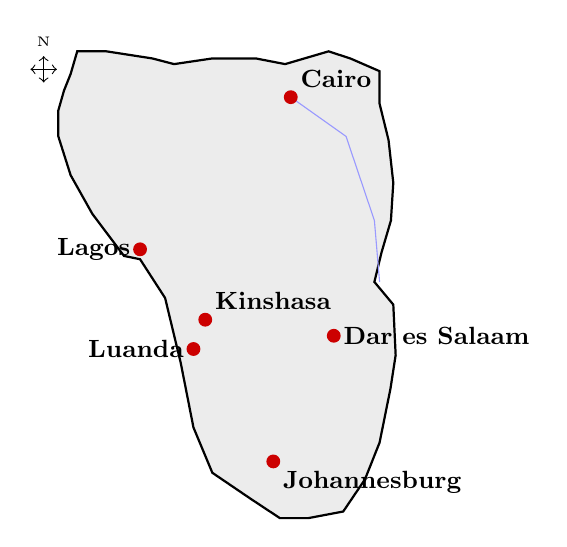
\begin{tikzpicture}[x=1cm, y=1cm, scale=0.6]
 % ---- Africa outline (simplified polygon) --------------------
  % Points traced roughly clockwise from Morocco/NW corner.
  % Coordinates are (x,y) in the projection above.
  \draw[thick, fill=gray!15] 
    % NW: Morocco/Western Sahara coast, then across North Africa
    (0.97, 9.40)  % Cape Spartel ~35.8N, 5.9W
    -- (1.11, 9.88) % Strait of Gibraltar area ~37N, 5W (slightly in)
    -- (1.73, 9.88) % ~37N, 10E (Tunisia/Algeria north)
    -- (2.70, 9.73) % ~36N, 10E Tunisia
    -- (3.16, 9.61) % ~35N, 11E
    -- (3.97, 9.73) % ~36N, 12E Libya
    -- (4.89, 9.73) % ~36N, 17E
    -- (5.51, 9.61) % ~35N, 20E Libya
    -- (6.43, 9.88) % ~37N, 25E (Crete area, just clip)
    -- (6.89, 9.73) % ~36N, 28E
    -- (7.51, 9.46) % ~34N, 31E Egypt north (Nile delta)
    -- (7.51, 8.77) % ~30N, 31E  (Cairo latitude)
    -- (7.70, 8.00) % ~27N, 33E Red Sea coast
    -- (7.80, 7.10) % ~22N, 34E
    -- (7.75, 6.30) % ~18N, 33E Sudan/Eritrea
    -- (7.55, 5.62) % ~14N, 32E (Horn direction)
    -- (7.40, 5.00) % ~11N, 31E Djibouti area
    -- (7.80, 4.52) % ~8N,  34E Ethiopia/Somalia horn
    -- (7.85, 3.45) % ~2N,  34E Kenya east
    -- (7.74, 2.74) % ~1S,  32E
    -- (7.51, 1.60) % ~10S, 31E Tanzania
    -- (7.20, 0.82) % ~17S, 30E Mozambique
    -- (6.74, 0.14) % ~24S, 27E
    -- (6.00, 0.00) % ~35S, 21E Cape area west
    -- (5.40, 0.00) % ~35S, 16E
    -- (4.78, 0.41) % ~30S, 11E Namibia
    -- (3.97, 0.96) % ~25S,  4E ... Namibia/Angola
    -- (3.57, 1.92) % ~18S,  2W Angola coast
    -- (3.30, 3.29) % ~10S, -1W Angola/Congo coast
    -- (2.97, 4.66) % ~0,   -2W Gabon
    -- (2.44, 5.48) % ~6N,  -5W Ivory Coast/Ghana
    -- (2.10, 5.55) % ~7N,  -8W Liberia
    -- (1.43, 6.44) % ~14N,-13W Guinea/Senegal
    -- (0.97, 7.26) % ~20N,-16W Mauritania
    -- (0.71, 8.08) % ~27N,-18W W. Sahara
    -- (0.71, 8.63) % ~31N,-18W
    -- (0.83, 9.05) % ~33N,-17W Morocco
    -- (0.97, 9.40) % back to start
  ;



  % ---- Nile suggested with thin line --------------------------
  \draw[blue!40, thin]
    (5.63, 8.91) -- (6.80, 8.08) -- (7.40, 6.30) -- (7.51, 5.00);

  % ---- City dots ----------------------------------------------
  \tikzstyle{city}=[circle, fill=red!80!black, inner sep=0pt,
                    minimum size=5pt]

  \node[city] (cairo)    at (5.63, 8.91) {};
  \node[city] (lagos)    at (2.44, 5.69) {};
  \node[city] (kinshasa) at (3.82, 4.20) {};
  \node[city] (luanda)   at (3.57, 3.58) {};
  \node[city] (dares)    at (6.54, 3.86) {};
  \node[city] (jhb)      at (5.26, 1.20) {};

  % ---- Labels (positioned to avoid overlap) ------------------
  \node[above right, font=\small\bfseries] at (cairo)    {Cairo};
  \node[left,        font=\small\bfseries] at (lagos)    {Lagos};
  \node[above right, font=\small\bfseries] at (kinshasa) {Kinshasa};
  \node[left,        font=\small\bfseries] at (luanda)   {Luanda};
  \node[right,       font=\small\bfseries] at (dares)    {Dar es Salaam};
  \node[below right, font=\small\bfseries] at (jhb)      {Johannesburg};

  % ---- Compass rose (simple) ----------------------------------
  \begin{scope}[shift={(0.4,9.5)}, scale=0.35]
    \draw[->] (0,0) -- (0, 0.8) node[above, font=\tiny]{N};
    \draw[->] (0,0) -- (0,-0.8);
    \draw[->] (0,0) -- ( 0.8,0);
    \draw[->] (0,0) -- (-0.8,0);
  \end{scope}

\end{tikzpicture}
\hfill
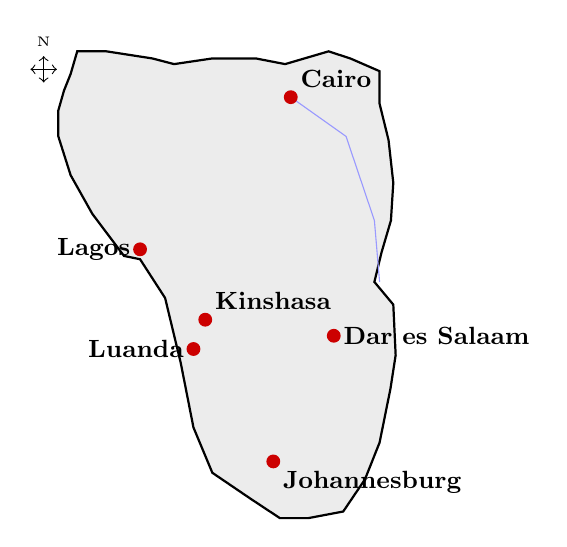
\begin{tikzpicture}[x=1cm, y=1cm, scale=0.6]
 % ---- Africa outline (simplified polygon) --------------------
  % Points traced roughly clockwise from Morocco/NW corner.
  % Coordinates are (x,y) in the projection above.
  \draw[thick, fill=gray!15] 
    % NW: Morocco/Western Sahara coast, then across North Africa
    (0.97, 9.40)  % Cape Spartel ~35.8N, 5.9W
    -- (1.11, 9.88) % Strait of Gibraltar area ~37N, 5W (slightly in)
    -- (1.73, 9.88) % ~37N, 10E (Tunisia/Algeria north)
    -- (2.70, 9.73) % ~36N, 10E Tunisia
    -- (3.16, 9.61) % ~35N, 11E
    -- (3.97, 9.73) % ~36N, 12E Libya
    -- (4.89, 9.73) % ~36N, 17E
    -- (5.51, 9.61) % ~35N, 20E Libya
    -- (6.43, 9.88) % ~37N, 25E (Crete area, just clip)
    -- (6.89, 9.73) % ~36N, 28E
    -- (7.51, 9.46) % ~34N, 31E Egypt north (Nile delta)
    -- (7.51, 8.77) % ~30N, 31E  (Cairo latitude)
    -- (7.70, 8.00) % ~27N, 33E Red Sea coast
    -- (7.80, 7.10) % ~22N, 34E
    -- (7.75, 6.30) % ~18N, 33E Sudan/Eritrea
    -- (7.55, 5.62) % ~14N, 32E (Horn direction)
    -- (7.40, 5.00) % ~11N, 31E Djibouti area
    -- (7.80, 4.52) % ~8N,  34E Ethiopia/Somalia horn
    -- (7.85, 3.45) % ~2N,  34E Kenya east
    -- (7.74, 2.74) % ~1S,  32E
    -- (7.51, 1.60) % ~10S, 31E Tanzania
    -- (7.20, 0.82) % ~17S, 30E Mozambique
    -- (6.74, 0.14) % ~24S, 27E
    -- (6.00, 0.00) % ~35S, 21E Cape area west
    -- (5.40, 0.00) % ~35S, 16E
    -- (4.78, 0.41) % ~30S, 11E Namibia
    -- (3.97, 0.96) % ~25S,  4E ... Namibia/Angola
    -- (3.57, 1.92) % ~18S,  2W Angola coast
    -- (3.30, 3.29) % ~10S, -1W Angola/Congo coast
    -- (2.97, 4.66) % ~0,   -2W Gabon
    -- (2.44, 5.48) % ~6N,  -5W Ivory Coast/Ghana
    -- (2.10, 5.55) % ~7N,  -8W Liberia
    -- (1.43, 6.44) % ~14N,-13W Guinea/Senegal
    -- (0.97, 7.26) % ~20N,-16W Mauritania
    -- (0.71, 8.08) % ~27N,-18W W. Sahara
    -- (0.71, 8.63) % ~31N,-18W
    -- (0.83, 9.05) % ~33N,-17W Morocco
    -- (0.97, 9.40) % back to start
  ;



  % ---- Nile suggested with thin line --------------------------
  \draw[blue!40, thin]
    (5.63, 8.91) -- (6.80, 8.08) -- (7.40, 6.30) -- (7.51, 5.00);

  % ---- City dots ----------------------------------------------
  \tikzstyle{city}=[circle, fill=red!80!black, inner sep=0pt,
                    minimum size=5pt]

  \node[city] (cairo)    at (5.63, 8.91) {};
  \node[city] (lagos)    at (2.44, 5.69) {};
  \node[city] (kinshasa) at (3.82, 4.20) {};
  \node[city] (luanda)   at (3.57, 3.58) {};
  \node[city] (dares)    at (6.54, 3.86) {};
  \node[city] (jhb)      at (5.26, 1.20) {};

  % ---- Labels (positioned to avoid overlap) ------------------
  \node[above right, font=\small\bfseries] at (cairo)    {Cairo};
  \node[left,        font=\small\bfseries] at (lagos)    {Lagos};
  \node[above right, font=\small\bfseries] at (kinshasa) {Kinshasa};
  \node[left,        font=\small\bfseries] at (luanda)   {Luanda};
  \node[right,       font=\small\bfseries] at (dares)    {Dar es Salaam};
  \node[below right, font=\small\bfseries] at (jhb)      {Johannesburg};

  % ---- Compass rose (simple) ----------------------------------
  \begin{scope}[shift={(0.4,9.5)}, scale=0.35]
    \draw[->] (0,0) -- (0, 0.8) node[above, font=\tiny]{N};
    \draw[->] (0,0) -- (0,-0.8);
    \draw[->] (0,0) -- ( 0.8,0);
    \draw[->] (0,0) -- (-0.8,0);
  \end{scope}

\end{tikzpicture}

\end{figure}
\vfill
\item Add weights to the edges of a complete graph on four vertices such that the Nearest Neighbor Algorithm starting at vertex A selects a Hamiltonian circuit that has very high weight.
\vfill
\end{enumerate}
\end{document}

%-------------------------------------------------------------------------------------------------------------------------------------------------------------------------------------------------------------------

%%% Local Variables:
%%% mode: latex
%%% TeX-master: t
%%% End:
